\documentclass[11pt,a4paper]{article}
			\usepackage[french]{babel}
					
				\usepackage{pifont}  
				\usepackage[utf8x]{inputenc}
				\usepackage[T1]{fontenc} 
				\usepackage{lmodern}			
				\usepackage{fancyhdr}
				\usepackage{textcomp}
				\usepackage{makeidx}
				\usepackage{tabularx}
				\usepackage{multicol}
				\usepackage{multirow}
				\usepackage{longtable}
				\usepackage{color}
				\usepackage{soul}
				\usepackage{boxedminipage}
				\usepackage{shadow}
				\usepackage{framed}			
				\usepackage{array}
				\usepackage{url}
				\usepackage{ragged2e}
				\usepackage{fancybox}
				\newcommand{\cadretitre}[2]{
				  \vspace*{0.8\baselineskip}
				  \begin{center}%
				  \boxput*(0,1){%
					%\colorbox{white}{\Large\textbf{\ #1\ }}%
				  }%
				  {%
					\setlength{\fboxsep}{10pt}%
				    \Ovalbox{\begin{minipage}{.8\linewidth}\begin{center}\Large\sffamily{#2}\end{center}\end{minipage}}}%
				  \end{center}
				  \vspace*{2\baselineskip}
				  }
			
			\makeatletter
			\def\@seccntformat#1{\protect\makebox[0pt][r]{\csname the#1\endcsname\quad}}
			\makeatother

				% Permet d'afficher qqchose à une positin absolue
				\usepackage[absolute]{textpos}
				\setlength{\TPHorizModule}{1cm}
				\setlength{\TPVertModule}{\TPHorizModule}
	
				\usepackage[titles]{tocloft}
				\setlength{\cftbeforesecskip}{0.5ex}
				\setlength{\cftbeforesubsecskip}{0.2ex}
				\addto\captionsfrench{\renewcommand\contentsname{}}
				
				\usepackage[font=scriptsize]{caption}
				
				\usepackage{listings}
\lstdefinestyle{lstverb}
  {
    basicstyle=\footnotesize,
    frameround=tttt, frame=trbl, framerule=0pt, rulecolor=\color{gray},
    lineskip=-1pt,   % pour rapprocher les lignes
    flexiblecolumns, escapechar=\\,
    tabsize=4, extendedchars=true
  }
\lstnewenvironment{Java}[1][]{\lstset{style=lstverb,language=java,#1}}{}
				\ifx\pdfoutput\undefined
					\usepackage{graphicx}
				\else
					\usepackage[pdftex]{graphicx}
				\fi
				\usepackage[a4paper, hyperfigures=true, colorlinks, linkcolor=black, citecolor=blue,urlcolor=blue, pagebackref=true, bookmarks=true, bookmarksopen=true,bookmarksnumbered=true,
                pdfauthor={}, pdftitle={TDLinux - Prise en main de l’environnement, rappels, linux avancé}, pdfkeywords={TDLinux - Prise en main de l'environnement, rappels, linux avanc\'e, },pdfpagemode=UseOutlines,pdfpagetransition=Dissolve,nesting=true,
				backref, pdffitwindow=true, bookmarksnumbered=true]{hyperref}
				\usepackage{supertabular}
				\usepackage[table]{xcolor}
				\usepackage{url}
				\usepackage{caption} 
				\setlength{\parskip}{1.3ex plus 0.2ex minus 0.2ex}
				\setlength{\parindent}{0pt}
				
				\makeatletter
				\def\url@leostyle{ \@ifundefined{selectfont}{\def\UrlFont{\sf}}{\def\UrlFont{\footnotesize\ttfamily}}}
				\makeatother
				\urlstyle{leo}
				
				\definecolor{examplecolor}{rgb}{0.156,0.333,0.443}
				\definecolor{definitioncolor}{rgb}{0.709,0.784,0.454}
				\definecolor{exercisecolor}{rgb}{0.49,0.639,0}
				\definecolor{hintcolor}{rgb}{0.941,0.674,0.196}
				\definecolor{tableHeadercolor}{rgb}{0.709,0.784,0.454}
				\definecolor{tablerowAltcolor}{rgb}{.866,.905,.737}
				\definecolor{tablerowAlt2color}{rgb}{.968,.976,.933}
				\definecolor{verylightgray}{rgb}{0.98,0.98,0.98}
				
				\newenvironment{fshaded}{
				\def\FrameCommand{\fcolorbox{framecolor}{shadecolor}}
				\MakeFramed {\FrameRestore}}
				{\endMakeFramed}
				
				\newenvironment{fexample}[1][]{\definecolor{shadecolor}{rgb}{.913,.913,.913}
				\definecolor{framecolor}{rgb}{.156,.333,.443}
				\begin{fshaded}}{\end{fshaded}} 
				
				\newenvironment{fdefinition}{\definecolor{shadecolor}{rgb}{.913,.913,.913}
				\definecolor{framecolor}{rgb}{.709,.784,.454}
				\begin{fshaded}}{\end{fshaded}}
				
				\newenvironment{fexercise}{\definecolor{shadecolor}{rgb}{.913,.913,.913}
				\definecolor{framecolor}{rgb}{.49,.639,0}
				\begin{fshaded}}{\end{fshaded}}
				
				\newenvironment{fhint}{\definecolor{shadecolor}{rgb}{.913,.913,.913}
				\definecolor{framecolor}{rgb}{.941,.674,.196}
				\begin{fshaded}}{\end{fshaded}}	
				
				\newcommand{\PreserveBackslash}[1]{
				\let\temp=\\#1\let\\=\temp
				}
				\let\PBS=\PreserveBackslash
				\newcolumntype{A}{>{\PBS\raggedright\small\hspace{0pt}}X}
				\newcolumntype{L}[1]{>{\PBS\raggedright\small\hspace{0pt}}p{#1}}
				\newcolumntype{R}[1]{>{\PBS\raggedleft\small\hspace{0pt}}p{#1}}
				\newcolumntype{C}[1]{>{\PBS\centering\small\hspace{0pt}}p{#1}}
				
				\makeindex
				
				\title{TDLinux - Prise en main de l'environnement, rappels, linux avanc\'e}	
			\date{}
			\author{\scriptsize{}}
			\definecolor{light-gray}{gray}{0.8}
			\renewcommand{\headrulewidth}{0pt}
			\fancyhead[L]{
				\footnotesize\textsc{Haute \'Ecole de Bruxelles}\\
	    			\footnotesize\textsc{\'Ecole Sup\'erieure d'Informatique}
			}
			\fancyhead[R]{
				\footnotesize{Bachelor en Informatique}\\
				\footnotesize{Laboratoires Java} - 
			\footnotesize{1\`ere ann\'ee}}
				\fancyfoot[L]{ }
				\fancyfoot[C]{}
				\fancyfoot[R]{\scriptsize{\textcolor{gray}{version 2014-2015 (\today)}}}
				\pagestyle{plain}
				\reversemarginpar
				\usepackage{rotating}						
				\begin{document}
					\begin{textblock}{9}(2,3.2)
						
\includegraphics[width=2cm]{../../../_templates/java/icons/logo-esi}
					\end{textblock}
				
				
				
				
				%\maketitle
				\cadretitre{TD1}{TDLinux - Prise en main de l'environnement, rappels, linux avanc\'e}
				\thispagestyle{fancy}
        \marginpar{\begin{sideways}
            \begin{minipage}[t]{1cm}
            \begin{tiny}
            
\includegraphics[width=1\linewidth,height=1\textheight,keepaspectratio=true]{../../../_templates/java/icons/cc-gris.jpg}
			\end{tiny}
			\end{minipage}
            \begin{minipage}[b]{19cm}
            \begin{tiny}
            \textcolor{gray}{Distribué sous licence Creative Commons Paternité - Partage à l'Identique 2.0 Belgique 
            (\texttt{http://creativecommons.org/licenses/by-sa/2.0/be/})
			\vspace{-1em}
			\\Les autorisations au-delà du champ de cette licence peuvent être obtenues à 
			\texttt{http://www.heb.be/esi}
			- \texttt{cleruste@heb.be}
			}\end{tiny}
			\end{minipage}
        \end{sideways}}
            \begin{abstract}
			Ce TD a pour but de vous rappeler les commandes 
			\verb@Linux@,
			des commandes de base aux commandes plus \'evolu\'ees.
		
            \par
        
  		Nous vous invitons \`a relire le Guide Visuel avant de commencer.
		
            \par
        \end{abstract}
				\vspace{-2em}\tableofcontents
				\pagestyle{plain}
            \clearpage
            \fancyhead[L,C,R]{}
            \fancyfoot[L,C]{}
            \fancyfoot[R]{ \scriptsize{\textcolor{gray}{
				TDLinux - page \thepage}}}
				\thispagestyle{fancy}
				\pagestyle{fancy}
	   
            \section{Les commandes de base de Linux}Revoyons ici les commandes de base\subsection{Les commandes de base}
					\begin{itemize}
				
			\item \,\verb|passwd|\, permet de \textbf{changer le mot de passe } ; 
        
			\item \,\verb|exit|\, permet de \textbf{quitter} ; 
        
			\item \,\verb|nano nomDuFichier|\, 
          permet d'\textbf{\'editer} le fichier 
          nomm\'e \textit{nomDuFichier} ; 
        
			\item \,\verb|cat nomDuFichier|\, 
          permet d'\textbf{afficher \`a l'\'ecran} le contenu du fichier 
          nomm\'e \textit{nomDuFichier} ; 
        
			\item \,\verb|ls|\, permet de \textbf{lister} le contenu d'un r\'epertoire ; 
        
			\item \,\verb|ls -a|\, permet de \textbf{lister} le contenu d'un r\'epertoire, y compris les fichiers cach\'es ; 
        
			\item \,\verb|ls -l|\, permet de \textbf{lister} le contenu d'un r\'epertoire au format long ; 
        
			\item \,\verb|mv nomDuFichier nouveauNomDuFichier|\, 
          permet de \textbf{renommer} le fichier nomm\'e \textit{nomDuFichier}
          en un fichier nomm\'e \textit{nouveauNomDuFichier} ; 
        
			\item \,\verb|mv nomDuFichier nomDuDossier|\, 
          permet de \textbf{d\'eplacer} le fichier nomm\'e \textit{nomDuFichier}
          dans un r\'epertoire nomm\'e \textit{nomDuDossier} ; 
        
			\item \,\verb|cp nomDuFichier nouveauNomDuFichier|\, 
          permet de \textbf{copier} le fichier nomm\'e \textit{nomDuFichier}
          en un fichier copie  nomm\'e \textit{nouveauNomDuFichier} situ\'e dans le m\^eme r\'epertoire; 
        
			\item \,\verb|cp nomDuFichier nomDuDossier|\, 
          permet de \textbf{copier} le fichier nomm\'e \textit{nomDuFichier}
          en un fichier copie  nomm\'e \textit{nomDuFichier} 
          situ\'e dans un r\'epertoire nomm\'e \textit{nomDuDossier} ; 
        
			\item \,\verb|rm nomDuFichier|\, 
          permet de \textbf{ d\'etruire } le fichier nomm\'e \textit{nomDuFichier}; 
        
			\item \,\verb|rmdir nomDuDossier|\, 
          permet de \textbf{d\'etruire} le dossier \textbf{vide} 
          nomm\'e \textit{nomDuDossier} ; 
        
			\item \,\verb|mkdir nomDuDossier|\, 
          permet de \textbf{cr\'eer un dossier vide} 
          nomm\'e \textit{nomDuDossier} ; 
        
			\item \,\verb|rm -r nomDuDossier|\, 
          permet de \textbf{d\'etruire} le dossier \textbf{pas forc\'ement vide} 
          nomm\'e \textit{nomDuDossier} ; 
        
			\item \,\verb|pwd|\, permet \textbf{d'afficher le chemin du dossier courant} 
          (celui o\`u vous \^etes en ce moment) ; 
        
			\item \,\verb|cd chemin/nomDuDossier|\, permet de changer le dossier 
          courant en \textit{chemin/nomDuDossier} ; 
        
			\item \,\verb|cd|\, permet de changer le dossier courant en votre dossier personnel ; 
        
					\end{itemize}
				\subsection{Les options dans la ligne de commande.}
				  Nous avons d\'ej\`a rencontr\'e l'une ou l'autre option ; 
				  par exemple, les options \,\verb|-a|\, 
				  ou \,\verb|-l|\, de \,\verb|ls|\, ;
				  ou encore l'option \,\verb|-r|\, de \,\verb|rm|\,.
        
            \par
        
				  Ces options modifient le sens d'une commande.
        
            \par
        
				  On les reconnait car elles commencent par un \,\verb|-|\, suivi d'une lettre
          ou \,\verb|--|\, suivi d'un nom d'option.
        
            \par
        
          Les options disponibles pour chaque commande se trouvent dans la page de manuel \,\verb|man|\, 
          de la commande en question.
				
            \par
        \subsection{Quelques commandes courantes}
			
		\subparagraph{Les commandes de base} 
		
                \textcolor{white}{.} \par
             
								La commande pour :  
							
					\begin{itemize}
				
			\item voir le contenu d'un dossier (la liste de ce qu'il contient) est  \textcolor{gray}{\underline{\hspace*{2em}}} 
			\item voir le contenu d'un dossier (la liste de ce qu'il contient) au format long est  \textcolor{gray}{\underline{\hspace*{3em}}} 
			\item voir le contenu d'un dossier (la liste de ce qu'il contient), y compris les fichiers cach\'es est  \textcolor{gray}{\underline{\hspace*{3em}}} 
			\item \'editer le contenu d'un fichier est  \textcolor{gray}{\underline{\hspace*{3em}}} 
			\item changer son mot de passe est  \textcolor{gray}{\underline{\hspace*{5em}}} 
			\item se d\'econnecter de linux1 est  \textcolor{gray}{\underline{\hspace*{3em}}} 
			\item copier un fichier est  \textcolor{gray}{\underline{\hspace*{2em}}} 
			\item renommer un fichier est  \textcolor{gray}{\underline{\hspace*{2em}}} 
			\item d\'eplacer un fichier est  \textcolor{gray}{\underline{\hspace*{2em}}} 
			\item changer de dossier courant est  \textcolor{gray}{\underline{\hspace*{2em}}} 
			\item cr\'eer un r\'epertoire est  \textcolor{gray}{\underline{\hspace*{3em}}} 
			\item visualiser le contenu d'un fichier sans l'\'editer est  \textcolor{gray}{\underline{\hspace*{2em}}} 
			\item voir quel est le dossier courant (son chemin) est  \textcolor{gray}{\underline{\hspace*{2em}}} 
			\item d\'etruire un fichier est  \textcolor{gray}{\underline{\hspace*{2em}}} 
			\item d\'etruire un dossier vide est  \textcolor{gray}{\underline{\hspace*{3em}}} 
			\item d\'etruire un dossier pas forc\'ement vide est  \textcolor{gray}{\underline{\hspace*{3em}}} 
			\item d'obtenir la liste des options de la commande rm est  \textcolor{gray}{\underline{\hspace*{5em}}} 
					\end{itemize}
				
			
		\subparagraph{La ligne de commande} 
		
                \textcolor{white}{.} \par
            
					\begin{itemize}
				
			\item 
										Qu'est-ce qui permet de distinguer / s\'eparer les diff\'erentes parties d'une commande ? 
										 \textcolor{gray}{\underline{\hspace*{10em}}} 
			\item 
										Dans la commande \,\verb|nanotest|\,, combien y a-t-il de parties ?  
										 \textcolor{gray}{\underline{\hspace*{1em}}} 
			\item 
										Dans la commande \,\verb|nano test|\,, combien y a-t-il de parties ?  
										 \textcolor{gray}{\underline{\hspace*{1em}}} 
					\end{itemize}
				\subsection{Ressources}\section{Syst\`eme de fichiers, chemin absolu et relatif}
				Nous allons maintenant nous rappeler ce qu'est le syst\`eme de fichiers et ce que sont les chemins absolus et relatifs.
			
            \par
        \subsection{Le syst\`eme de fichiers}\begin{figure}[hbt]
				    \begin{center}
					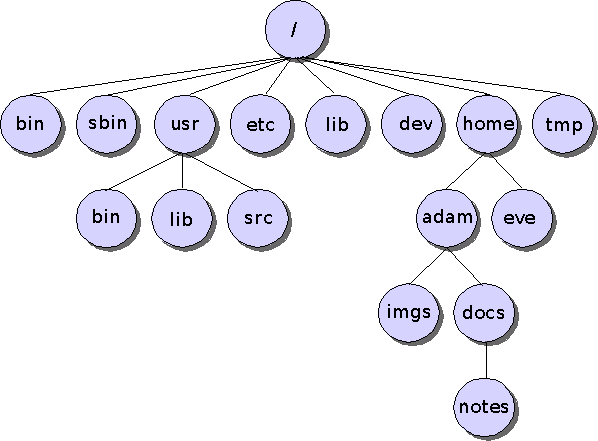
\includegraphics[width=0.8\linewidth,height=0.8\textheight,keepaspectratio=true]{/home/cuvelier/Documents/ESI/Java/2016-2017/DEV1Q2/notes/DEV1Q2/TDLinux/fr/image/arborescenceUnix.png}
						\end{center}
                
                    \caption[arborescenceUnix.png]{arborescenceUnix.png}
                \end{figure}
                    
			    
			    [source : franceftars.us.62-152-34-99.ppa.listkom.ru]
        
            \par
        
			    Chaque utilisateur dispose d'un dossier personnel, par exemple ici \,\verb|adam|\, et \,\verb|eve|\,
			    qui se trouve dans un dossier appel\'e home, qui se trouve lui-m\^eme dans un dossier appel\'e / (la barre oblique). 
        
            \par
        
			    / est le dossier principal (on dit aussi la racine) du syst\`eme de fichiers.
        
            \par
        
			    Avec Linux, tous les syst\`emes de fichiers sont assembl\'es en un seul syst\`eme de fichiers dont le dossier principal est d\'esign\'e par la barre oblique (/).
        
            \par
        
          On peut voir que le dossier principal (\,\verb|/|\,) contient le dossier \,\verb|home|\, 
          qui contient le dossier \,\verb|adam|\,, 
          la home de l'utilisateur \,\verb|adam|\,.
        
            \par
        
          Attention ! Le dossier appel\'e \,\verb|home|\, ne contient pas que la home de l'utilisateur mais toutes les homes.
        
            \par
        
          Ici, il contient aussi le dossier \,\verb|eve|\, qui est la home de l'utilisateur \,\verb|eve|\,.
        
            \par
        
          Il y a des notations de r\'epertoires particuliers :
          
					\begin{itemize}
				
			\item le r\'epertoire \,\verb|.|\, qui repr\'esente le dossier courant ;
			\item le r\'epertoire \,\verb|..|\, qui repr\'esente le dossier parent ;
			\item le r\'epertoire \,\verb|~|\, qui repr\'esente le dossier personnel, 
			        c'est un raccourci pour la home de l'utilisateur, c-\`a-d, par exemple \,\verb|~|\, vaut \,\verb|/home/adam|\, 
			        si l'utilisateur a pour home \,\verb|/home/adam|\, .
					\end{itemize}
				
          Supposons \^etre l'utilisateur \,\verb|adam|\, dans le dossier courant \,\verb|adam|\,, 
          
					\begin{itemize}
				
			\item \,\verb|ls ~|\, liste le contenu du r\'epertoire \,\verb|adam|\,, 
			        il est ici \'equivalent \`a la commande \,\verb|ls|\,  ;
            
			\item \,\verb|ls .|\, liste le contenu du r\'epertoire \,\verb|adam|\,, 
			        il est ici \'equivalent \`a la commande \,\verb|ls|\,  ;
            
			\item \,\verb|ls ..|\, liste le contenu du r\'epertoire parent de \,\verb|adam|\,, 
			        c-\`a-d \,\verb|home|\,.
            
					\end{itemize}
				
            \par
        
          Supposons \^etre l'utilisateur \,\verb|adam|\, dans le dossier courant \,\verb|notes|\,, 
          
					\begin{itemize}
				
			\item \,\verb|ls ~|\, liste le contenu du r\'epertoire \,\verb|adam|\, ;
            
			\item \,\verb|ls .|\, liste le contenu du r\'epertoire \,\verb|notes|\,, 
			        il est ici \'equivalent \`a la commande \,\verb|ls|\,  ;
            
			\item \,\verb|ls ..|\, liste le contenu du r\'epertoire parent de \,\verb|notes|\,, 
			        c-\`a-d \,\verb|docs|\,.
            
					\end{itemize}
				
            \par
        \subsection{Chemin relatif}\begin{figure}[hbt]
				    \begin{center}
					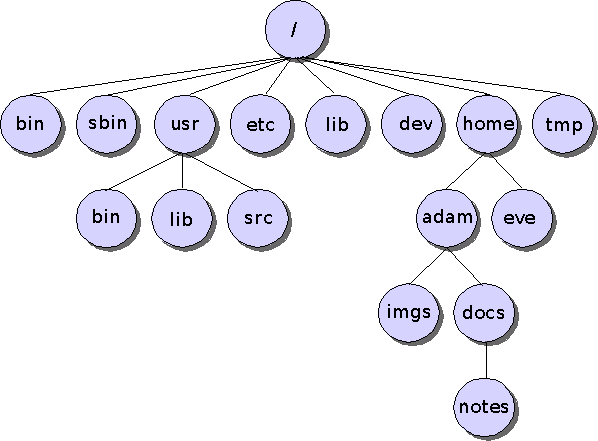
\includegraphics[width=0.8\linewidth,height=0.8\textheight,keepaspectratio=true]{/home/cuvelier/Documents/ESI/Java/2016-2017/DEV1Q2/notes/DEV1Q2/TDLinux/fr/image/arborescenceUnix.png}
						\end{center}
                
                    \caption[arborescenceUnix.png]{arborescenceUnix.png}
                \end{figure}
                    
			    
			    [source : franceftars.us.62-152-34-99.ppa.listkom.ru]
        
            \par
        
        Si on se trouve dans la home de l'utilisateur \,\verb|adam|\, et qu'on veut lister le contenu du r\'epertoire \,\verb|notes|\,,
        
					\begin{itemize}
				
			\item 
            on peut le faire en 2 \'etapes en changeant de r\'epertoire courant :
            \,\verb|cd docs|\,\,\verb|ls notes|\,
			\item 
            on peut aussi le faire sans changer de r\'epertoire courant, 
            il faut alors lui indiquer le chemin pour arriver au fichier :
            \,\verb|ls docs/notes|\,
					\end{itemize}
				
        On parle de  \textbf{chemin relatif} car on va indiquer le chemin \`a suivre \`a partir du dossier courant,
        en effet, \textbf{\`a partir du dossier}\,\verb|adam|\,,
        on va dans le dossier \,\verb|docs|\,, puis, on va lister le dossier \,\verb|notes|\,.
        
            \par
        \subsection{Chemin absolu}\begin{figure}[hbt]
				    \begin{center}
					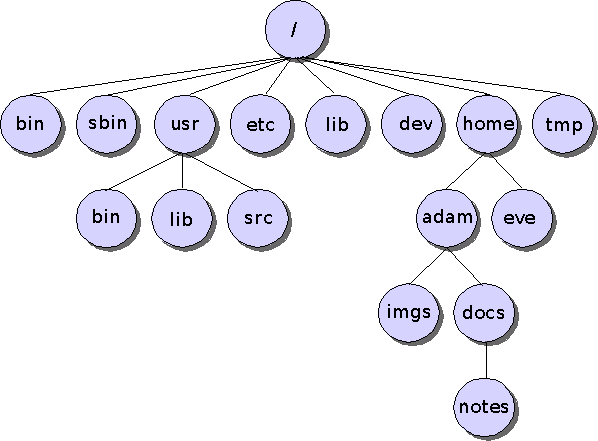
\includegraphics[width=0.8\linewidth,height=0.8\textheight,keepaspectratio=true]{/home/cuvelier/Documents/ESI/Java/2016-2017/DEV1Q2/notes/DEV1Q2/TDLinux/fr/image/arborescenceUnix.png}
						\end{center}
                
                    \caption[arborescenceUnix.png]{arborescenceUnix.png}
                \end{figure}
                    
			    
			    [source : franceftars.us.62-152-34-99.ppa.listkom.ru]
        
            \par
        
        Si on se trouve dans la home de l'utilisateur \,\verb|adam|\, et qu'on veut lister le contenu du r\'epertoire \,\verb|notes|\,,
        
					\begin{itemize}
				
			\item 
            on peut aussi le faire sans changer de r\'epertoire courant, 
            en lui indiquant le chemin pour arriver au fichier \`a partir de la racine :
            \,\verb|ls /home/adam/docs/notes|\,
					\end{itemize}
				
        On parle de  \textbf{chemin absolu} car on va indiquer le chemin \`a suivre \textbf{\`a partir de la racine},
        cette commande fonctionne donc peu importe le dossier courant.
        
            \par
        \subsection{Exercices}
			
		\subparagraph{} 
		
                \textcolor{white}{.} \par
            La racine du syst\`eme de fichier sous Linux est
						
            \begin{itemize} 
        
            \item[ \ding{"6D} ] .
        
            \item[ \ding{"6D} ] ..
        
            \item[ \ding{"6D} ] \char`\~
        
            \item[ \ding{"6D} ] \char`\~g12345
        
            \item[ \ding{"6D} ] /
        
            \item[ \ding{"6D} ] /home
        
            \end{itemize} 
        
			
		\subparagraph{} 
		
                \textcolor{white}{.} \par
            Le(s)quel(s) de ces chemins est/sont un chemin absolu ?
						
            \begin{itemize} 
        
            \item[ \ding{"6F} ] /home/g54321/tdLinux
        
            \item[ \ding{"6F} ] \char`\~g54321/tdLinux
        
            \item[ \ding{"6F} ] g54321/tdLinux
        
            \item[ \ding{"6F} ] tdLinux
        
            \end{itemize} 
        
			
		\subparagraph{} 
		
                \textcolor{white}{.} \par
            Le(s)quel(s) de ces chemins est/sont un chemin relatif ?
						
            \begin{itemize} 
        
            \item[ \ding{"6F} ] tdLinux
        
            \item[ \ding{"6F} ] ../tdLinux
        
            \item[ \ding{"6F} ] ./.././eCours/tdLinux
        
            \item[ \ding{"6F} ] /eCours/java/tds/tdLinux
        
            \end{itemize} 
        \begin{figure}[hbt]
				    \begin{center}
					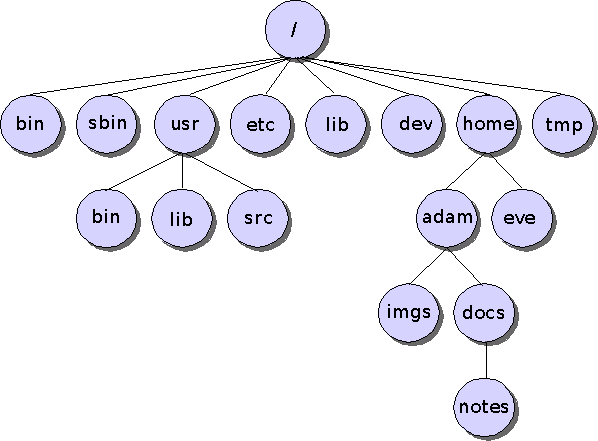
\includegraphics[width=0.8\linewidth,height=0.8\textheight,keepaspectratio=true]{/home/cuvelier/Documents/ESI/Java/2016-2017/DEV1Q2/notes/DEV1Q2/TDLinux/fr/image/arborescenceUnix.png}
						\end{center}
                
                    \caption[arborescenceUnix.png]{arborescenceUnix.png}
                \end{figure}
                    
			    
			    [source : franceftars.us.62-152-34-99.ppa.listkom.ru]
        
            \par
        
			
		\subparagraph{La ligne de commande} 
		
                \textcolor{white}{.} \par
            
							Supposons que le r\'epertoire courant est le dossier personnel \,\verb|/home/adam|\,
					\begin{itemize}
				
			\item 
										Quelle commande permet de supprimer le r\'epertoire \,\verb|imgs|\, et son contenu en utilisant un chemin absolu ?
										 \textcolor{gray}{\underline{\hspace*{16em}}} 
			\item 
										Quelle commande permet de supprimer le r\'epertoire \,\verb|imgs|\, et son contenu en utilisant un chemin relatif ?
										 \textcolor{gray}{\underline{\hspace*{10em}}} 
			\item 
										Quelle commande permet de cr\'eer un r\'epertoire \,\verb|imgs|\, 
										dans le r\'epertoire \,\verb|eve|\, en utilisant un chemin relatif ?
										 \textcolor{gray}{\underline{\hspace*{16em}}} 
			\item 
										Quelle commande permet de cr\'eer un fichier \,\verb|mesImages|\, 
										dans le r\'epertoire \,\verb|imgs|\, du r\'epertoire \,\verb|eve|\, en utilisant un chemin absolu ?
										 \textcolor{gray}{\underline{\hspace*{16em}}} 
			\item 
										Quelle commande permet de copier ce fichier \,\verb|mesImages|\, 
										que vous venez de cr\'eer dans le r\'epertoire courant en utilisant que des chemins relatifs ?
										 \textcolor{gray}{\underline{\hspace*{16em}}} 
					\end{itemize}
				\begin{figure}[hbt]
				    \begin{center}
					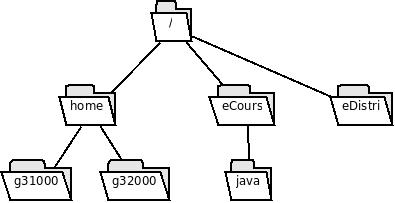
\includegraphics[width=0.8\linewidth,height=0.8\textheight,keepaspectratio=true]{/home/cuvelier/Documents/ESI/Java/2016-2017/DEV1Q2/notes/DEV1Q2/TDLinux/fr/image/fs.jpeg}
						\end{center}
                
                    \caption[fs.jpeg]{fs.jpeg}
                \end{figure}
                    
            \par
        
			
		\subparagraph{La ligne de commande} 
		
                \textcolor{white}{.} \par
            
							Supposons que le r\'epertoire courant est le dossier personnel \verb@/home/g31000@
					\begin{itemize}
				
			\item 
										Quelle commande permet de supprimer le r\'epertoire \verb@java@ et son contenu en utilisant un chemin absolu ?
										 \textcolor{gray}{\underline{\hspace*{16em}}} 
			\item 
										Quelle commande permet de supprimer le r\'epertoire \verb@java@ et son contenu en utilisant un chemin relatif ?
										 \textcolor{gray}{\underline{\hspace*{16em}}} 
			\item 
										Quelle commande permet de cr\'eer un r\'epertoire \verb@tds@ 
										dans le r\'epertoire \verb@g32000@ en utilisant un chemin relatif ?
										 \textcolor{gray}{\underline{\hspace*{16em}}} 
			\item 
										Quelle commande permet de cr\'eer un fichier \verb@Ex.java@ 
										dans le r\'epertoire \verb@tds@ 
										du r\'epertoire \verb@g32000@ en utilisant un chemin relatif ?
										 \textcolor{gray}{\underline{\hspace*{16em}}} 
			\item 
										Quelle commande permet de copier ce fichier \verb@Ex.java@ 
										que vous venez de cr\'eer dans le r\'epertoire courant en utilisant que des chemins relatifs ?
										 \textcolor{gray}{\underline{\hspace*{16em}}} 
			\item 
										Quelle commande permet de lister au format long le dossier personnel en utilisant un chemin absolu ?
										 \textcolor{gray}{\underline{\hspace*{5em}}} 
					\end{itemize}
				\section{La ligne de commande}\subsection{La ligne de commande}
          Parfois, vous devez entrer une commande assez longue parce que les noms de fichiers sont longs et/ou nombreux.
          Linux offre plusieurs facilit\'es pour simplifier l'entr\'ee de longues commandes.  
        
            \par
        
			
		\subparagraph{La compl\'etion de la commande} 
		
					\textcolor{white}{.} \par
				
            \par
        
          Lorsque vous appuyez sur la touche \,\verb|TAB|\,,
          le shell tente de compl\'eter le d\'ebut de commande que vous avez d\'ej\`a tap\'e.
          Si plusieurs possibilit\'es existent, elles sont affich\'ees si vous appuyez 2x sur  \,\verb|TAB|\,.  
        
            \par
        
			
		\subparagraph{Exp\'erience} 
		
					\textcolor{white}{.} \par
				
            \par
          
          Supposons que vous ne vous rappeliez plus tr\`es bien de la commande qui permet de modifier le mot de passe.
          Vous vous rappelez juste qu'elle commence par \,\verb|pas|\,.  
        
            \par
        
					\begin{enumerate}
				
			\item 
			  Tapez \,\verb|pas|\,  
			  puis appuyez 2x sur la touche \,\verb|TAB|\,.
			\item 
			Entrez un \,\verb|s|\,  
            puis appuyez \`a nouveau sur \,\verb|TAB|\,.
          
					\end{enumerate}
				
			
		\subparagraph{La compl\'etion des noms de fichiers} 
		
					\textcolor{white}{.} \par
				
            \par
        
          La touche de tabulation permet \'egalement de compl\'eter un nom de fichier. 
        
            \par
        
			
		\subparagraph{Exercice} 
		
					\textcolor{white}{.} \par
				
            \par
        
					\begin{enumerate}
				
			\item 
            Dans votre dossier td3, copiez le fichier \par
				\verb@monfichieraunomtellementlongquilmeparaitpeuprobabledeletaper2xsanserreur@
            qui se trouve dans le dossier \verb@/eCours/java/td/td3@.
          
			\item Affichez le contenu de ce fichier en \'evitant de retaper son nom.
					\end{enumerate}
				
			
		\subparagraph{Joker} 
		
					\textcolor{white}{.} \par
				
            \par
        
          Il faut savoir que beaucoup de commandes linux qui traitent un fichier peuvent en traiter plusieurs \`a la fois; il suffit de les indiquer tous.
        
            \par
        
          Par exemple : \,\verb|rm texte1 texte2 texte3 texte4|\, supprime les 4 fichiers indiqu\'es.
        
            \par
        
          On voudrait aller plus loin et \'eviter de taper explicitement chaque nom. Par exemple, on pourrait avoir envie de dire :
          
					\begin{enumerate}
				
			\item Supprime tous les fichiers qui commencent par \guillemotleft  texte \guillemotright  ;
			\item Supprime tous les fichiers Java (qui se terminent par .java) ;
			\item ...
					\end{enumerate}
				
          C'est possible gr\^ace \`a la notion de \guillemotleft  joker \guillemotright . 
          On ne va pas donner explicitement un nom de fichier mais un \guillemotleft  motif \guillemotright , c'est-\`a-dire une description des noms de fichiers concern\'es.
        
            \par
        
          Il y a essentiellement deux jokers : 
          
					\begin{itemize}
				
			\item \,\verb|?|\, : lorsque le bash rencontre un \verb@?@ 
            dans un nom de fichier il sait qu'il peut le remplacer par n'importe quel caract\`ere ;
          
			\item 
            et \,\verb|*|\, : lorsque le bash rencontre un \verb@*'@ 
            dans un nom de fichier il sait qu'il peut le remplacer par n'importe quelle suite de caract\`eres  (0, 1 ou plusieurs caract\`eres).
          
					\end{itemize}
				
            \par
        
			
		\subparagraph{Exercices} 
		
					\textcolor{white}{.} \par
				
            \par
        
					\begin{enumerate}
				
			\item 
            Copiez dans votre r\'epertoire td3 tous les fichiers du r\'epertoire 
            \verb@/eCours/java/td/td3@ dont la deuxi\`eme lettre est un '\verb@x@'.
          
			\item 
            Copiez dans votre r\'epertoire tdLinux tous les fichiers du r\'epertoire
            \verb@/eCours/java/td/td3@ dont l'extension est \verb@.java@ 
            (c'est possible sans passer par un \,\verb|cd /eCours/java/td/td3|\,)
          
			\item 
            Listez le contenu des r\'epertoires des \'etudiants (pour rappel, les r\'epertoires des \'etudiants sont ceux 
            qui se trouvent dans \verb@/home@ et qui commencent par un '\verb@g@').
          
			\item 
            Listez le contenu des r\'epertoires des professeurs (pour rappel, les  
            r\'epertoires des professeurs sont ceux qui se trouvent dans \verb@/home@ et qui sont compos\'es de 3 lettres).
          
					\end{enumerate}
				
			
		\subparagraph{S\'election multiple} 
		
                \textcolor{white}{.} \par
            La commande \verb@rm td*.java@ supprime le(s) fichier(s) :
						
            \begin{itemize} 
        
            \item[ \ding{"6F} ]  
							td.java
						
        
            \item[ \ding{"6F} ]  
							td2
						
        
            \item[ \ding{"6F} ]  
							td2.java
						
        
            \item[ \ding{"6F} ]  
							td3Prepa.java
						
        
            \item[ \ding{"6F} ]  
							td3.java
						
        
            \item[ \ding{"6F} ]  
							td10.java
						
        
            \end{itemize} 
        
			
		\subparagraph{} 
		
                \textcolor{white}{.} \par
            La commande \verb@rm td?.java@ supprime le(s) fichier(s) :
						
            \begin{itemize} 
        
            \item[ \ding{"6F} ]  
              td.java
						
        
            \item[ \ding{"6F} ]  
							td2
						
        
            \item[ \ding{"6F} ]  
							td2.java
						
        
            \item[ \ding{"6F} ]  
							td3Prepa.java
						
        
            \item[ \ding{"6F} ]  
							td3.java
						
        
            \item[ \ding{"6F} ]  
							td10.java
						
        
            \end{itemize} 
        
			
		\subparagraph{Revenir \`a une commande pr\'ec\'edente} 
		
					\textcolor{white}{.} \par
				
            \par
          
          Il arrive souvent qu'il faille entrer une commande qu'on a d\'ej\`a \'ecrite il y a peu (ou en tout cas fort proche de ce qu'on a d\'ej\`a \'ecrit). 
          C'est l\`a que les fl\`eches viennent \`a notre secours.  
        
            \par
          
          La fl\`eche vers le haut permet de revenir aux commandes pr\'ec\'edentes et de les modifier. \`A utiliser sans mod\'eration...  
        
            \par
        \section{Les permissions}\subsection{Les groupes d'un utilisateur}
					Les utilisateurs d'un syst\`eme Linux sont group\'es. 
					Un groupe contient un ou plusieurs utilisateur(s) et un utilisateur appartient \`a un ou plusieurs groupe(s).
				
            \par
        
				  Sur Linux1, 
        
            \par
        \begin{figure}[hbt]
				    \begin{center}
					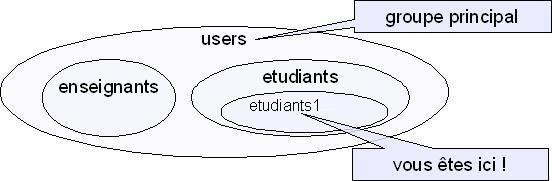
\includegraphics[width=0.8\linewidth,height=0.8\textheight,keepaspectratio=true]{/home/cuvelier/Documents/ESI/Java/2016-2017/DEV1Q2/notes/DEV1Q2/TDLinux/fr/image/groupesLinux1.jpg}
						\end{center}
                
                    \caption[groupesLinux1.jpg]{groupesLinux1.jpg}
                \end{figure}
                    
            \par
        
					\begin{itemize}
				
			\item users : tous les utilisateurs sont dans ce groupe
			\item enseignants : tous les professeurs sont dans ce groupe
			\item etudiants : tous les \'etudiants sont dans ce groupe
			\item etudiants1 : tous les \'etudiants de premi\`ere ann\'ee sont dans ce groupe
					\end{itemize}
				
            \par
        
				  La commande \,\verb|groups|\, permet de connaitre tous les groupes 
				  auxquels l'utilisateur appartient.
				
            \par
        
				  Parmi tous les groupes d'un utilisateur, il y en a un qui est le groupe principal (c'est le premier donn\'e par la commande \,\verb|groups|\,). 
				  C'est celui qui sera utilis\'e par d\'efaut lors de certaines op\'erations (par exemple, lors de la cr\'eation d'un fichier)
				
            \par
        \subsection{Propri\'etaire et groupe d'un fichier}
					Tous les fichiers ont un propri\'etaire et appartiennent \`a un groupe.
					C'est la base pour d\'efinir les permissions sur ce fichier.
					On pourra ainsi donner des permissions diff\'erentes :
					
					\begin{itemize}
				
			\item au propri\'etaire du fichier ;
			\item aux utilisateurs qui appartiennent au m\^eme groupe que le fichier ;
			\item  \`a tous les autres. 
					\end{itemize}
				
            \par
        
				  Lister au format long le contenu du r\'epertoire nous permet de voir les infos suivantes :
				
            \par
        \begin{figure}[hbt]
				    \begin{center}
					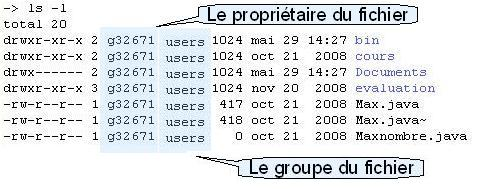
\includegraphics[width=0.8\linewidth,height=0.8\textheight,keepaspectratio=true]{/home/cuvelier/Documents/ESI/Java/2016-2017/DEV1Q2/notes/DEV1Q2/TDLinux/fr/image/permissions.jpg}
						\end{center}
                
                    \caption[permissions.jpg]{permissions.jpg}
                \end{figure}
                    
            \par
        
          Sur le sch\'ema ci-dessus, on peut lire, par exemple, que le fichier \verb@Max.java@ 
          appartient \`a \verb@g32671@ et a \'et\'e plac\'e dans le groupe users.
        
            \par
        
          Nous vous disions qu'il existait un groupe principal (le premier donn\'e par la commande \,\verb|groups|\,)
          et que c'est celui qui serait utilis\'e par d\'efaut lors de certaines op\'erations.
        
            \par
        
          C'est le cas par exemple ici,
          quand l'utilisateur \verb@g32671@ a cr\'e\'e son fichier \verb@Max.java@,
          ce fichier s'est retrouv\'e dans le groupe par d\'efaut \verb@users@.
        
            \par
        
          Or, 
        
            \par
        \begin{figure}[hbt]
				    \begin{center}
					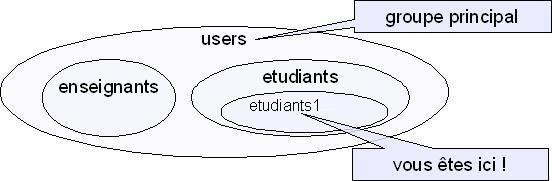
\includegraphics[width=0.8\linewidth,height=0.8\textheight,keepaspectratio=true]{/home/cuvelier/Documents/ESI/Java/2016-2017/DEV1Q2/notes/DEV1Q2/TDLinux/fr/image/groupesLinux1.jpg}
						\end{center}
                
                    \caption[groupesLinux1.jpg]{groupesLinux1.jpg}
                \end{figure}
                    
            \par
        
          le groupe \,\verb|users|\, contient \`a la fois 
          le groupe \,\verb|étudiants|\,/\,\verb|étudiants1|\, et
          aussi le groupe \,\verb|enseignants|\,.
        
            \par
        
					Comme nous avons vu que nous pouvions donner des permissions diff\'erentes :
					
					\begin{itemize}
				
			\item au propri\'etaire du fichier ;
			\item aux utilisateurs qui appartiennent au m\^eme groupe que le fichier ;
			\item  \`a tous les autres. 
					\end{itemize}
				
          Si le groupe du fichier est \verb@users@, 
          les utilisateurs qui appartiennent au m\^eme groupe que le fichier sont \`a la fois
          des \,\verb|étudiants|\,/\,\verb|étudiants1|\, 
          et des \,\verb|enseignants|\,.
        
            \par
        
           On ne pourrait donc pas distinguer les permissions des \'etudiants de celles des enseignants.
				
            \par
        
				  Pour faire la distinction entre \'etudiants et enseignants, il faudrait changer le groupe auquel appartient le fichier.
				
            \par
        \,\verb|chgrp etudiants1 Max.java|\, indique que le fichier \verb@Max.java@ doit \^etre plac\'e dans le
				  groupe \verb@etudiants1@ (le propri\'etaire du fichier peut ex\'ecuter cette commande mais il doit obligatoirement indiquer un groupe auquel il appartient).
				
            \par
        
				  Il existe aussi une commande que seul l'administrateur peut ex\'ecuter \,\verb|chown g32000 Max.java|\, 
				  qui change le propri\'etaire du fichier\verb@ Max.java@ \`a \verb@g32000@.
        
            \par
        
			
		\subparagraph{Exercices} 
		
					\textcolor{white}{.} \par
				
            \par
        
					\begin{enumerate}
				
			\item Visualisez le propri\'etaire des fichiers de votre dossier personnel.
			\item Cr\'eez un r\'epertoire \verb@tdLinux@ dans votre dossier personnel ;
			\item Visualisez le propri\'etaire des fichiers de votre dossier \verb@tdLinux@.
					
					\end{enumerate}
				
			
		\subparagraph{Exercices} 
		
					\textcolor{white}{.} \par
				
            \par
        
					\begin{enumerate}
				
			\item Visualiser les groupes auxquels vous appartenez.
			\item Visualiser le groupe auquel appartient votre dossier \verb@tdLinux@.
			\item Quel est votre groupe principal ? 
			\item Quels sont les groupes auxquels appartient votre professeur ?
			\item Avez-vous un groupe en commun avec lui ?
			\item Quel(s) groupe(s) Linux avez-vous en commun avec les autres \'etudiants de votre groupe ESI ?
			\item Changez le groupe de  votre dossier \verb@tdLinux@ 
					pour que les enseignants puissent avoir des permissions diff\'erentes de celles des \'etudiants .
					\end{enumerate}
				
			
		\subparagraph{Exercices} 
		
					\textcolor{white}{.} \par
				
            \par
        
					\begin{enumerate}
				
			\item Visualisez vos fichiers et d\'eterminez \`a quel groupe ils appartiennent.
			\item Cr\'eez un fichier de test et modifiez le groupe auquel il appartient.
					\end{enumerate}
				
			
		\subparagraph{FAQ} 
		
					\textcolor{white}{.} \par
				
            \par
        \textbf{Les fichiers dans mon dossier personnel ne sont pas automatiquement \`a moi ?}
            \par
          
					Non. En pratique c'est g\'en\'eralement le cas, 
					mais on peut tr\`es bien trouver dans un dossier personnel un fichier qui appartient \`a quelqu'un d'autre.  
				
            \par
        \subsection{Les permissions}
			
		\subparagraph{Les permissions sur un fichier} 
		
					\textcolor{white}{.} \par
				
            \par
        
					Vous savez qu'un fichier appartient \`a un utilisateur et est plac\'e dans un groupe.
				
            \par
        
					Vous savez aussi que vous pouvez donner des permissions diff\'erentes :
					
					\begin{itemize}
				
			\item au propri\'etaire du fichier ;
			\item aux utilisateurs qui appartiennent au m\^eme groupe que le fichier ;
			\item  \`a tous les autres. 
					\end{itemize}
				
            \par
        
					Voyons maintenant quelles sont ces permissions.
					Il existe 3 types de permissions : en lecture, en \'ecriture et en ex\'ecution.
					
					\begin{itemize}
				
			\item Lecture : si une personne a le droit en lecture sur un fichier, il peut en voir le contenu. Par exemple, avec cat, more ou encore view.
			\item \'Ecriture : Si une personne a le droit en \'ecriture sur un fichier, il peut en modifier le contenu. Par exemple, avec nano.
			\item Ex\'ecution : Cette permission concerne les ex\'ecutables. Un ex\'ecutable est un fichier qui contient un programme en langage machine directement ex\'ecutable par le processeur.
					\end{itemize}
				
          Ces 3 permissions peuvent \'evidemment \^etre combin\'ees (exemple : on donne l'acc\`es en lecture ET en \'ecriture). 
				
            \par
        
				  En pratique, on ne veut pas donner les m\^emes droits \`a tout le monde. On pourra pr\'eciser :
				  
					\begin{itemize}
				
			\item les droits du propri\'etaire d'un fichier ;
			\item les droits des utilisateurs qui appartiennent au m\^eme groupe que le fichier ;
			\item les droits pour toutes les personnes non reprises dans une cat\'egorie ci-dessus (les autres).
					\end{itemize}
				
            \par
        
				  Lister au format long le contenu du r\'epertoire nous permet de voir les infos suivantes :
				
            \par
        \begin{figure}[hbt]
				    \begin{center}
					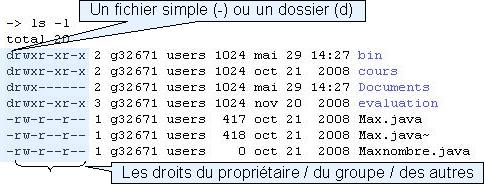
\includegraphics[width=0.8\linewidth,height=0.8\textheight,keepaspectratio=true]{/home/cuvelier/Documents/ESI/Java/2016-2017/DEV1Q2/notes/DEV1Q2/TDLinux/fr/image/permissions2.jpg}
						\end{center}
                
                    \caption[permissions2.jpg]{permissions2.jpg}
                \end{figure}
                    
            \par
        
          Les permissions sont indiqu\'ees avec des lettres (r pour la lecture, w pour l'\'ecriture et x pour l'ex\'ecution) 
          dans cet ordre en mettant un tiret (-) si la permission n'est pas donn\'ee. 
        
            \par
        
          Il y a 3 blocs de 3 donn\'ees pour les droits du propri\'etaire, des utilisateurs du groupe auquel le fichier est attribu\'e et enfin, des autres (dans cet ordre).
        
            \par
        
          Sur l'exemple ci-dessus, on peut voir que le fichier\verb@ Max.java@ :
          
					\begin{itemize}
				
			\item est en lecture/\'ecriture pour le propri\'etaire (g32671) ; 
			\item est en lecture seule pour tous les utilisateurs du groupe users (en fait tout le monde sur linux1) ; 
			\item est en lecture seule pour les autres (en fait personne sur linux1).
					\end{itemize}
				
            \par
        
			
		\subparagraph{Les permissions sur un r\'epertoire.} 
		
					\textcolor{white}{.} \par
				
            \par
        
					Tout comme pour les fichiers, on peut donner des permissions au dossier.
        
            \par
        
					  La situation est sensiblement la m\^eme : 
					  
					\begin{itemize}
				
			\item un dossier a un propri\'etaire et un groupe ;
			\item on indique les m\^emes permissions r, w et x ;
			\item on sp\'ecifie des permissions pour le propri\'etaire, le groupe et les autres.
					\end{itemize}
				
            \par
        
          Ce qui change, c'est la signification des permissions. Que veut dire \guillemotleft  ex\'ecuter \guillemotright  un dossier par exemple ?
				
            \par
        
					Explicitons \`a pr\'esent le sens de chaque droit :
					 
					\begin{itemize}
				
			\item lecture : on a le droit de lister le contenu du dossier, de voir ce qu'ilcontient. On peut par exemple faire un ls du dossier.
			\item \'ecriture : on peut modifier le contenu du dossier. On peut ainsi effacer un fichier (via la commande rm).
					    On remarque ainsi que pour effacer un fichier il ne faut pas de droit en \'ecriture sur le fichier mais bien sur le dossier qui le contient.
			\item ex\'ecution : on peut \guillemotleft  ouvrir \guillemotright  le dossier / entrer dedans. 
					    On peut ainsi en faire son dossier courant (cd td1) ou le traverser dans un chemin (cat td1/monTexte1).
					\end{itemize}
				
            \par
        
			
		\subparagraph{Changer les permissions.} 
		
					\textcolor{white}{.} \par
				
            \par
        
					Lorsqu'un fichier est cr\'e\'e, il l'est avec des permissions par d\'efaut d\'efinies par l'administrateur du syst\`eme.
				
            \par
        
				  On peut \'evidemment les changer via la commande \,\verb|chmod|\,.
				
            \par
        
				  Il existe 2 notations fort diff\'erentes pour indiquer les permissions : avec un nombre et avec des lettres.
				
            \par
        
			
		\subparagraph{Changer les permissions avec un nombre.} 
		
					\textcolor{white}{.} \par
				
            \par
        
				  Pour changer les permissions avec un nombre, vous donnez d'un coup toutes les permissions que vous autorisez 
				  
					\begin{itemize}
				
			\item d'abord, au propri\'etaire du dossier/fichier ;
			\item ensuite, aux utilisateurs qui appartiennent au m\^eme groupe que le dossier/fichier ;
			\item enfin, \`a tous les autres. 
					\end{itemize}
				
          Vous avez vu qu'il y a une permission de lecture, d'\'ecriture et d'ex\'ecuter/de traverser.
          Si vous avez fait un peu attention, vous aurez remarqu\'e que chacune de ces permissions se situe dans un ordre bien pr\'ecis :
          
					\begin{itemize}
				
			\item d'abord une permission de lecture (r) ;
			\item ensuite une permission d'\'ecrire (w) ;
			\item enfin une permission d'ex\'ecuter/de traverser (x). 
					\end{itemize}
				\,\verb|rwx|\, avec \`a chaque fois la possibilit\'e ou non d'avoir cette permission.
				
            \par
        
				  On pourrait 
				  
					\begin{itemize}
				
			\item 
              avoir uniquement un droit de lecture : \,\verb|r--|\, 
              qu'on pourrait \'ecrire \,\verb|100|\,
              et convertir en 4 (100 en base 2)
            
			\item 
              avoir uniquement un droit d'\'ecriture : \,\verb|-w-|\, 
              qu'on pourrait \'ecrire \,\verb|010|\,
              et convertir en 2 (010 en base 2)
            
			\item 
              avoir uniquement un droit d'ex\'ecution/de traverser : \,\verb|--x|\, 
              qu'on pourrait \'ecrire \,\verb|001|\,
              et convertir en 1 (001 en base 2)
            
			\item 
              avoir un droit de lecture et d'\'ecriture : \,\verb|rw-|\, 
              qu'on pourrait \'ecrire \,\verb|110|\,
              et convertir en 6 (110 en base 2)
            
			\item 
              avoir un droit de lecture et d'ex\'ecution/de traverser : \,\verb|r-x|\, 
              qu'on pourrait \'ecrire \,\verb|101|\,
              et convertir en 5 (101 en base 2)
            
			\item 
              avoir un droit d'\'ecriture et d'ex\'ecution/de traverser : \,\verb|-wx|\, 
              qu'on pourrait \'ecrire \,\verb|011|\,
              et convertir en 3 (011 en base 2)
            
			\item 
              avoir tous les droits (de lecture, d'\'ecriture et d'ex\'ecution/de traverser) : \,\verb|rwx|\, 
              qu'on pourrait \'ecrire \,\verb|111|\,
              et convertir en 7 (111 en base 2)
            
			\item 
              avoir n'avoir aucun droit (ni de lecture, ni d'\'ecriture ni d'ex\'ecution/de traverser) : \,\verb|---|\, 
              qu'on pourrait \'ecrire \,\verb|000|\,
              et convertir en 0 (000 en base 2)
            
					\end{itemize}
				
				C'est ce nombre trouv\'e pour les permissions qu'on donnera 
				
					\begin{itemize}
				
			\item d'abord, au propri\'etaire du dossier/fichier ;
			\item ensuite, aux utilisateurs qui appartiennent au m\^eme groupe que le dossier/fichier ;
			\item enfin, \`a tous les autres. 
					\end{itemize}
				
          On combine alors les nombres obtenus pour les 3 sortes d'utilisateurs.
				
            \par
        \,\verb|chmod 640 monFichier.java|\, donne 
				  
					\begin{itemize}
				
			\item au propri\'etaire le droit en lecture/\'ecriture ;
			\item aux utilisateurs dans le m\^eme groupe que le fichier le droit en lecture uniquement ; 
			\item et aucun droit aux autres.
					\end{itemize}
				
            \par
        
			
		\subparagraph{Changer les permissions avec des lettres.} 
		
					\textcolor{white}{.} \par
				
            \par
        
				  Pour changer les permissions avec des lettres, vous dites les permissions que vous ajoutez/retirez, \`a qui vous les ajoutez/retirez et ce,sans toucher aux autres droits.
				  
					\begin{itemize}
				
			\item 
					    Il faut d'abord dire \`a qui on modifie les droits :
					    
					\begin{itemize}
				
			\item \verb@u@ pour le propri\'etaire \textit{(user)}
			\item \verb@g@ pour le groupe auquel le fichier/dossier appartient \textit{(group)}
			\item \verb@o@ pour les autres \textit{(other)}
			\item \verb@a@ pour tous (le propri\'etaire, le groupe auquel le fichier/dossier appartient, les autres) \textit{(all)}
					\end{itemize}
				
			\item 
              ensuite, sp\'ecifier 
              
					\begin{itemize}
				
			\item \verb@+@ si on ajoute des droits ;
			\item \verb@-@ si on en retire.
					\end{itemize}
				
			\item 
              On indique enfin quel(s) droit(s) on ajoute ou enl\`eve 
                
					\begin{itemize}
				
			\item r
			\item w
			\item x
					\end{itemize}
				
					\end{itemize}
				
            \par
        \,\verb|chmod a+w monFichier.java|\,
					\begin{itemize}
				
			\item ajoute
			\item le droit d'\'ecriture
			\item \`a tous
					\end{itemize}
				
          pour le fichier \verb@monFichier.java@.
        
            \par
        \,\verb|chmod go-wx monFichier.exe|\,
					\begin{itemize}
				
			\item retire
			\item les droits d'\'ecriture et d'ex\'ecution
			\item aux utilisateurs du m\^eme groupe que celui auquel appartient le fichier et aux autres (c-\`a-d \`a tout lemonde sauf le propri\'etaire)
					\end{itemize}
				
          pour le fichier \verb@monFichier.exe@.
        
            \par
        
			
		\subparagraph{D\'eterminez les bonnes permissions} 
		
                \textcolor{white}{.} \par
              
							Remplissez les blancs avec la permission correcte (r, w, x ou -). 
							Il s'agit de trouver la permission minimale \`a mettre pour r\'epondre \`a la demande.   
						
					\begin{itemize}
				
			\item 
									Pour un fichier Java, la permission la plus ad\'equate est
									 \textcolor{gray}{\underline{\hspace*{1em}}}  \textcolor{gray}{\underline{\hspace*{1em}}}  \textcolor{gray}{\underline{\hspace*{1em}}} 
			\item 
									Pour la version compil\'ee (le bytecode), la permission la plus ad\'equate est
									 \textcolor{gray}{\underline{\hspace*{1em}}}  \textcolor{gray}{\underline{\hspace*{1em}}}  \textcolor{gray}{\underline{\hspace*{1em}}} 
			\item 
									Le fichier qui contient (l'ex\'ecutable de) la machine virtuelle a probablement comme permisson
									 \textcolor{gray}{\underline{\hspace*{1em}}}  \textcolor{gray}{\underline{\hspace*{1em}}}  \textcolor{gray}{\underline{\hspace*{1em}}} 
					\end{itemize}
				
			
		\subparagraph{Exercice } 
		
					\textcolor{white}{.} \par
				
            \par
          
					Soit le fichier \verb@Max.java@ de la capture d'\'ecran ci-dessous.  
				
            \par
        \begin{figure}[hbt]
				    \begin{center}
					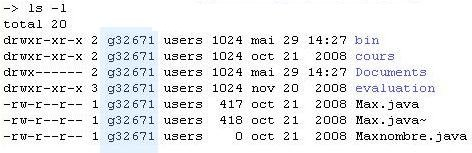
\includegraphics[width=0.8\linewidth,height=0.8\textheight,keepaspectratio=true]{/home/cuvelier/Documents/ESI/Java/2016-2017/DEV1Q2/notes/DEV1Q2/TDLinux/fr/image/ls-l.jpg}
						\end{center}
                
                    \caption[Contenu d\'etaill\'e d'un dossier]{Contenu d\'etaill\'e d'un dossier}
                \end{figure}
                    
					Est-ce qu'un professeur peut l'\'editer ? 
				
            \par
        \fcolorbox{gray}{verylightgray}{\parbox{\textwidth}{\textcolor{verylightgray}{\LARGE  Non ! Le droit d'écriture n'est accordé qu'au propriétaire.  }}} {\footnotesize\emph{(la r\'eponse est disponible dans la version en ligne)}\par} 
			
		\subparagraph{D\'eterminez les bonnes permissions} 
		
                \textcolor{white}{.} \par
            
							Soit le fichier "Max.java" de la capture d'\'ecran ci-dessus.
							
							On voudrait que l'\'etudiant \verb@g32671@ puisse travailler  
							normalement, que les autres \'etudiants ne puissent pas tricher sur  
							lui mais que les professeurs puissent lire son travail.   
						
					\begin{itemize}
				
			\item 
									Quel groupe faut-il donner au fichier ?
									\par
				 \textcolor{gray}{\underline{\hspace*{10em}}} 
			\item 
									Quelle commande permet de donner ce groupe au fichier ?
									\par
				 \textcolor{gray}{\underline{\hspace*{3em}}}  \textcolor{gray}{\underline{\hspace*{10em}}}  \textcolor{gray}{\underline{\hspace*{10em}}} 
			\item 
									Quelles permissions minimales donner au fichier ?                
									\par
				 \textcolor{gray}{\underline{\hspace*{1em}}}  \textcolor{gray}{\underline{\hspace*{1em}}}  \textcolor{gray}{\underline{\hspace*{1em}}}  \textcolor{gray}{\underline{\hspace*{1em}}}  \textcolor{gray}{\underline{\hspace*{1em}}}  \textcolor{gray}{\underline{\hspace*{1em}}}  \textcolor{gray}{\underline{\hspace*{1em}}}  \textcolor{gray}{\underline{\hspace*{1em}}}  \textcolor{gray}{\underline{\hspace*{1em}}} 
			\item 
									Quelle commande permet de donner ces permissions au fichier ?
									\par
				 \textcolor{gray}{\underline{\hspace*{3em}}}  \textcolor{gray}{\underline{\hspace*{2em}}}  \textcolor{gray}{\underline{\hspace*{10em}}} 
					\end{itemize}
				
			
		\subparagraph{Exercice} 
		
					\textcolor{white}{.} \par
				
            \par
          
					Reprenez les permissions affich\'ees dans la capture d'\'ecran ci-dessous 
					et exprimez-les avec un nombre de 3 chiffres.  
				
            \par
        \begin{figure}[hbt]
				    \begin{center}
					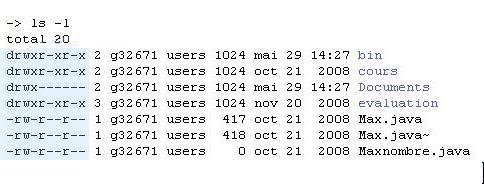
\includegraphics[width=0.8\linewidth,height=0.8\textheight,keepaspectratio=true]{/home/cuvelier/Documents/ESI/Java/2016-2017/DEV1Q2/notes/DEV1Q2/TDLinux/fr/image/ls-l-permissions.jpg}
						\end{center}
                
                    \caption[Contenu d\'etaill\'e d'un dossier]{Contenu d\'etaill\'e d'un dossier}
                \end{figure}
                    \clearpage
			
		\subparagraph{Permissions par d\'efaut} 
		
					\textcolor{white}{.} \par
				
            \par
        
					\begin{enumerate}
				
			\item Si ce n'est pas encore fait, cr\'eez un dossier "tdLinux".
			\item Cr\'eez-y un fichier vide.
			\item Demandez les d\'etails du fichier (propri\'etaire, groupe, permission)
					\end{enumerate}
				 
					On constate qu'un nouveau fichier appartient \`a celui qui l'a cr\'e\'e 
					(on s'en doute) et au groupe principal du cr\'eateur. 
					Il y a aussi des permissions par d\'efaut (plut\^ot permissives dans notre cas).  
				
            \par
        
			
		\subparagraph{Modifier les permissions} 
		
					\textcolor{white}{.} \par
				
            \par
          
					Vous savez que la commande qui permet de modifier les permissions d'un fichier est 
					\,\verb|chmod|\,.  
				
            \par
          
					Prenez le temps de \textbf{lire} 
					la page de \textbf{manuel} de cette commande.   
				
            \par
        
			
		\subparagraph{Exercices} 
		
					\textcolor{white}{.} \par
				
            \par
        
					\begin{enumerate}
				
			\item Cr\'eez un fichier \verb@brol@ dans le dossier \verb@tdLinux@ avec quelques mots.
			\item Faites en sorte que personne d'autre ne puisse en voir le contenu.
			\item Faites en sorte que tout le monde puisse voir son contenu mais pas le modifier. 
			\item 
					  Faites en sorte que les autres \'etudiants ne puissent pas voir son contenu mais les professeurs bien. 
					  Attention, pour ce faire, il faut pouvoir distinguer les \'etudiants des enseignants; et donc, distinguer les groupes.
					
					\end{enumerate}
				
			
		\subparagraph{Exercices} 
		
					\textcolor{white}{.} \par
				
            \par
          
					Modifiez les droits de votre dossier \verb@tdLinux@ et, si n\'ecessaire, 
					des fichiers qui s'y trouvent pour que tout le monde puisse  
				
            \par
        
					\begin{enumerate}
				
			\item voir quels fichiers s'y trouvent mais sans pouvoir lire le contenu de ces fichiers;
			\item modifier le contenu d'un des fichiers mais pas supprimer ce fichier;
			\item supprimer un fichier mais pas modifier son contenu.
					\end{enumerate}
				
			
		\subparagraph{Les commandes linux} 
		
                \textcolor{white}{.} \par
            Quelle commande linux permet de faire l'action suivante ?
					\begin{itemize}
				
			\item se d\'econnecter  \textcolor{gray}{\underline{\hspace*{3em}}} 
			\item changer son mot de passe  \textcolor{gray}{\underline{\hspace*{5em}}} 
			\item nettoyer l'\'ecran  \textcolor{gray}{\underline{\hspace*{3em}}} 
			\item voir le contenu d'un dossier au format long
									 \textcolor{gray}{\underline{\hspace*{2em}}}  \textcolor{gray}{\underline{\hspace*{2em}}} 
			\item cr\'eer un r\'epertoire  \textcolor{gray}{\underline{\hspace*{3em}}} 
			\item d\'eplacer un fichier  \textcolor{gray}{\underline{\hspace*{2em}}} 
			\item connaitre les groupes d'un utilisateur  \textcolor{gray}{\underline{\hspace*{5em}}} 
			\item modifier le groupe d'un fichier  \textcolor{gray}{\underline{\hspace*{3em}}} 
			\item modifier le propri\'etaire d'un fichier (par le super-utilisateur!)         
									 \textcolor{gray}{\underline{\hspace*{3em}}} 
			\item 
								  retirer la permission de traverser le r\'epertoire 
									\verb@tds@ \`a tous       
									 \textcolor{gray}{\underline{\hspace*{3em}}}  \textcolor{gray}{\underline{\hspace*{2em}}}  \textcolor{gray}{\underline{\hspace*{2em}}} 
			\item 
								  placer le fichier \verb@Hello.java@ 
									dans le groupe \verb@etudiants1@ \textcolor{gray}{\underline{\hspace*{3em}}}  \textcolor{gray}{\underline{\hspace*{10em}}}  \textcolor{gray}{\underline{\hspace*{10em}}} 
					\end{itemize}
				
			
		\subparagraph{Les permissions} 
		
                \textcolor{white}{.} \par
            Remplissez les blancs avec la permission minimale correcte (r, w, x ou -),
					\begin{enumerate}
				
			\item 
									pour que le r\'epertoire \verb@/home/gxxxxx/td3@ 
									permette \`a un autre \'etudiant d'y cr\'eer le fichier  
									\verb@/home/gxxxxx/td3/fichier@\par
				 \textcolor{gray}{\underline{\hspace*{1em}}}  \textcolor{gray}{\underline{\hspace*{1em}}}  \textcolor{gray}{\underline{\hspace*{1em}}}  \textcolor{gray}{\underline{\hspace*{1em}}}  \textcolor{gray}{\underline{\hspace*{1em}}}  \textcolor{gray}{\underline{\hspace*{1em}}}  \textcolor{gray}{\underline{\hspace*{1em}}}  \textcolor{gray}{\underline{\hspace*{1em}}}  \textcolor{gray}{\underline{\hspace*{1em}}} 
			\item 
									pour que le r\'epertoire \verb@/home/gxxxxx/td3@ 
									permette \`a un autre \'etudiant d'acc\'eder au fichier  
									\verb@/home/gxxxxx/td3/fichier@
									dont il connait le chemin
									\par
				 \textcolor{gray}{\underline{\hspace*{1em}}}  \textcolor{gray}{\underline{\hspace*{1em}}}  \textcolor{gray}{\underline{\hspace*{1em}}}  \textcolor{gray}{\underline{\hspace*{1em}}}  \textcolor{gray}{\underline{\hspace*{1em}}}  \textcolor{gray}{\underline{\hspace*{1em}}}  \textcolor{gray}{\underline{\hspace*{1em}}}  \textcolor{gray}{\underline{\hspace*{1em}}}  \textcolor{gray}{\underline{\hspace*{1em}}} 
					\end{enumerate}
				
			
		\subparagraph{} 
		
                \textcolor{white}{.} \par
            Modifiez les permissions 
					\begin{itemize}
				
			\item 
									pour que le fichier \verb@/home/gxxxxx/td3/fichier@ 
									puisse \^etre lu et modifi\'e par votre professeur et vous m\^eme mais seulement lu par les autres \'etudiants 
									\par
				 \textcolor{gray}{\underline{\hspace*{3em}}}  \textcolor{gray}{\underline{\hspace*{1em}}}  \textcolor{gray}{\underline{\hspace*{1em}}}  \textcolor{gray}{\underline{\hspace*{1em}}}  \textcolor{gray}{\underline{\hspace*{16em}}} 
			\item 
								  \`A quel groupe ce fichier doit-il appartenir ?
									\par
				 \textcolor{gray}{\underline{\hspace*{10em}}} 
			\item 
								  Quelle commande permet de modifier le groupe du fichier afin de l'adapter \`a ce qui est demand\'e ci-dessus ?
									\par
				 \textcolor{gray}{\underline{\hspace*{3em}}}  \textcolor{gray}{\underline{\hspace*{10em}}} 
					\end{itemize}
				
			
		\subparagraph{S\'election multiple} 
		
                \textcolor{white}{.} \par
            Parmi les propositions suivantes, lesquelles repr\'esentent des chemins absolus ?
            \begin{itemize} 
        
            \item[ \ding{"6F} ] \verb@/usr/local/java/@
        
            \item[ \ding{"6F} ] \verb@/home/g31000/td3@
        
            \item[ \ding{"6F} ] \verb@g31000/td3@
        
            \item[ \ding{"6F} ] \verb@~/td3@
        
            \item[ \ding{"6F} ] \verb@td3@
        
            \item[ \ding{"6F} ] \verb@~g31000/td3@
        
            \end{itemize} 
        \section{Compter (wc)}\subsection{Compter (wc)}
					Vous vous demandez peut-\^etre
					combien de lignes fait un programme
					que vous avez \'ecrit
					ou encore 
					combien de lignes vous avez \'ecrites aujourd'hui.
					La commande 
					\verb@wc@
					peut vous r\'epondre ;
					elle indique le nombre de lignes,
					de mots et de caract\`eres
					contenus dans les fichiers donn\'es.
					\par
				
					Syntaxe : 
					\,\verb|wc fichier...|\,
            \par
        
			
		\subparagraph{Exemple} 
		
					\textcolor{white}{.} \par
				
					La commande : 
					\,\verb|wc Ex2.java|\,
					affiche le nombre de lignes, mots et caract\`eres
					contenus dans le fichier
					\verb@Ex2.java@.
				
            \par
        
			
		\subparagraph{Exercices} 
		
					\textcolor{white}{.} \par
				
					\begin{enumerate}
				
			\item 
							Comment afficher le nombres de lignes
							de tous les fichiers Java de votre dossier courant.
						
			\item 
							Examinez les options de la commande
							et trouvez comment n'afficher
							\textbf{que}
							le nombre de lignes
							et pas le nombre de mots et de caract\`eres.
						
			\item 
							Une convention d'\'ecriture Java
							indique de ne pas d\'epasser la
							colonne 80 dans les programmes.
							Trouvez l'option qui permet de
							v\'erifier que tous vos programmes
							actuels v\'erifient cette convention.
						
					\end{enumerate}
				
			\fcolorbox{gray}{verylightgray}{
			\begin{minipage}[c][3cm][c]{\textwidth}\textcolor{verylightgray}{X}\end{minipage}
		}\par\medskip
            \par
        \section{Recherche dans des fichiers (grep)}\subsection{Recherche dans des fichiers (grep)}
					Il est parfois difficile de s'y retrouver dans les fichiers.
					Vous allez \^etre amen\'es \`a vous poser des questions du genre :
				
            \par
        
					\begin{itemize}
				
			\item 
						Dans quel fichier ai-je \'ecrit un programme qui v\'erifie si une ann\'ee est bissextile ?
					
			\item 
						Dans quel fichier ai-je d\'ej\`a utilis\'e un switch ?
					
					\end{itemize}
				
					La commande \verb@grep@ peut venir \`a votre secours.
					Dans son utilisation la plus simple, elle permet d'extraire de fichiers
					toutes les lignes qui contiennent un certain texte (appel\'e 
					\textit{pattern}).
					\par
				
					Syntaxe : 
					\,\verb|grep pattern fichier...|\,
            \par
        
			
		\subparagraph{Exemple} 
		
					\textcolor{white}{.} \par
				
					Pour trouver dans quel fichier vous avez utilis\'e une variable nomm\'ee "bissextile",
					vous pouvez \'ecrire :
					\par
				\par
				\,\verb|grep bissextile *.java|\,
            \par
        
			
		\subparagraph{Exercices} 
		
					\textcolor{white}{.} \par
				
					\begin{enumerate}
				
			\item 
							Comment trouver les programmes Java
							du TD4
							o\`u vous avez d\'ej\`a utilis\'e un "switch" ?
						
			\item 
							Comment trouver,
							parmi \textbf{tous}
							les programmes Java
							que vous avez d\'ej\`a \'ecrits,
							ceux qui utilisent des bool\'eens ?
						
					\end{enumerate}
				
			\fcolorbox{gray}{verylightgray}{
			\begin{minipage}[c][2cm][c]{\textwidth}\textcolor{verylightgray}{X}\end{minipage}
		}\par\medskip
            \par
        \section{Recherche de fichier (find)}\subsection{Recherche de fichier (find)}\verb@find@ est une commande linux 
				tr\`es puissante qui vous fera gagner beaucoup de temps.
				Elle permet de rechercher dans une arborescence de fichiers 
				ceux qui correspondent \`a un crit\`ere donn\'e 
				(taille, droits, nom, dates...).
				Elle permet \'egalement d'appliquer une commande \`a chacun 
				des fichiers ainsi trouv\'es.
			
            \par
        
				Attention \`a ne pas la confondre
				avec la commande
				\verb@grep@
				qui va examiner le contenu des fichiers.
			
            \par
        
			
		\subparagraph{Exemple} 
		
					\textcolor{white}{.} \par
				
            \par
        \begin{Java}
find ~ -name Ex.java
			\end{Java}
				Recherche, chez vous 
				(\verb@~@),
				un fichier nomm\'e 
				\verb@Ex.java@
            \par
        
			
		\subparagraph{Exercice} 
		
					\textcolor{white}{.} \par
				
            \par
        
				Trouvez avec la commande 
				\verb@find@
				tous les fichiers Java que vous avez d\'ej\`a \'ecrits.
			
            \par
        
			\fcolorbox{gray}{verylightgray}{
			\begin{minipage}[c][1cm][c]{\textwidth}\textcolor{verylightgray}{X}\end{minipage}
		}\par\medskip
				Nous avons \'ecrit pour vous une classe
				\verb@Color@
				mais nous ne savons plus tr\`es bien
				o\`u nous l'avons stock\'ee.
				Nous nous rappelons juste l'avoir mise
				quelque part dans 
				\verb@/eCours@.
				Pouvez-vous la retrouver pour nous ?
			
            \par
        
			\fcolorbox{gray}{verylightgray}{
			\begin{minipage}[c][1cm][c]{\textwidth}\textcolor{verylightgray}{X}\end{minipage}
		}\par\medskip\section{Redirections}\subsection{Entr\'ees et sorties standards}
			\begin{boxedminipage}[h]{\linewidth}
		
						Tout programme qui s'ex\'ecute dispose 
						de trois fichiers ouverts d'office 
						par le syst\`eme pour lui :
						l'entr\'ee standard, la sortie standard et la sortie d'erreur,
						identifi\'es respectivement par les num\'eros 0, 1 et 2.
					
            \par
        
						En Java, on retrouve ces trois fichiers :
					
            \par
        
					\begin{itemize}
				
			\item \verb@System.in@
						pour 0 (entr\'ee standard) 
						qu'on retrouve dans la d\'eclaration
						\verb@Scanner clavier = new Scanner(System.in);@
			\item \verb@System.out@
						pour 1 (sortie standard) 
						qu'on retrouve dans l'instruction
						\verb@System.out.println();@
			\item \verb@System.err@
						pour 2 (erreur standard) 
						qu'on retrouve dans l'instruction
						\verb@System.err.println();@
					\end{itemize}
				
			\end{boxedminipage}

					Cela peut vous paraitre bizarre de dire
					que le clavier et l'\'ecran sont des fichiers
					mais c'est bien ainsi que le programme
					les voit.
					Et c'est pratique,
					car nous allons pouvoir
					\textit{rediriger}
					ces entr\'ees et ces sorties vers de vrais fichiers
					de fa\c con tout \`a fait transparente pour le
					programme ; il ne sera pas n\'ecessaire de le modifier.
				
            \par
        \subsection{Rediriger la sortie}
					Il est possible,
					au moment o\`u on lance un programme,
					de rediriger sa sortie.
					Tout ce que le programme enverra
					sur sa sortie standard
					(par exemple avec un
					\verb@System.out.println()@
					en Java) ne sera pas visible \`a l'\'ecran
					mais sera envoy\'e dans, par exemple, un fichier.
				
            \par
        
			\begin{boxedminipage}[h]{\linewidth}
		
					Une redirection de sortie standard se note 
					\guillemotleft >\guillemotright  ou \guillemotleft 1>\guillemotright  lors du lancement du programme.
					Ces redirections sont r\'ealis\'ees par le shell avant 
					l'ex\'ecution de la commande 
					et sont transparentes pour cette commande.
				
			\end{boxedminipage}

			
		\subparagraph{Exemple} 
		
					\textcolor{white}{.} \par
				
            \par
        \begin{Java}
ls -l > liste
\end{Java}
					ou
				\begin{Java}
ls -l 1> liste
\end{Java}
					Ces deux commandes sont \'equivalentes;
					elles n'affichent pas le r\'esultat \`a l'\'ecran,
					mais l'\'ecrivent dans le fichier 
					\verb@liste@ cr\'e\'e ici ou \'ecras\'e 
					s'il pr\'eexistait.
					Par d\'efaut \verb@ls -l@ 
					affiche le r\'esultat \`a l'\'ecran.
					Nous avons \textit{redirig\'e} 
					cette sortie standard vers un fichier, 
					en l'occurrence \verb@liste@.
				
            \par
        
					Faites l'essai et v\'erifiez le contenu du fichier cr\'e\'e.
				
            \par
        
			
		\subparagraph{Exercice} 
		
					\textcolor{white}{.} \par
				
            \par
        
					\begin{enumerate}
				
			\item 
						Reprenez votre programme qui affiche
						des suites de nombres et plus pr\'ecis\'ement
						celui qui affiche la suite appel\'ee :
						"le pas croissant".
						Ex\'ecutez-le pour
						afficher les 1000 premiers nombres de cette suite.
					
			\item 
						Sauvez le r\'esultat dans un fichier
						pour pouvoir l'examiner \`a votre aise.
						\textbf{Rappel} :
						pour examiner le contenu d'un fichier,
						inutile de passer par un \'editeur,
						la commande
						\verb@more@
						suffit.
					
			\item 
						Est-ce que le nombre 15007 en fait partie ?
						(aide : vous vous rappelez de la commande
						\verb@grep@ ?)
					
					\end{enumerate}
				
			
		\subparagraph{Note} 
		
					\textcolor{white}{.} \par
				
            \par
        
					Avec la simple redirection en sortie, 
					si le fichier existe d\'ej\`a, il est \'ecras\'e. 
					Nous pouvons choisir de ne pas l'\'ecraser, 
					mais de le compl\'eter 
					(ajouter du contenu \`a la fin du fichier) 
					via la double redirection (en sortie) not\'ee 
					\verb@>>@.			
				
            \par
        \subsection{Rediriger l'entr\'ee}
					L'\guillemotleft entr\'ee standard\guillemotright  peut \^etre associ\'ee \`a un 
					fichier au lieu du clavier.
					Cela permet d'utiliser les donn\'ees \`a partir du fichier 
					au lieu de les entrer au clavier.
					C'est ce qu'on appelle une redirection de l'entr\'ee.
				
            \par
        
			\begin{boxedminipage}[h]{\linewidth}
		
					La redirection d'entr\'ee se note \guillemotleft <\guillemotright .			
				
			\end{boxedminipage}

			
		\subparagraph{Exemple} 
		
					\textcolor{white}{.} \par
				
            \par
        \verb@commande < data@\par
				
					Les lectures de la commande se feront dans
					le fichier \verb@data@
					et pas au clavier.
				
            \par
        
			
		\subparagraph{Exp\'erimentation} 
		
					\textcolor{white}{.} \par
				
            \par
        
						Nous avons \'ecrit pour vous une petite classe
						\verb@Multiples5@
						qui lit une s\'erie de nombres et n'affiche
						que ceux qui sont des multiples de 5.
						\`A la fin, elle affiche le nombre de multiples de 5.
					
            \par
        
					\begin{enumerate}
				
			\item 
						Copiez-la chez vous ; vous la trouverez
						quelque part dans \verb@/eCours/java@.
					
			\item 
						Lancez l'application et entrez des nombres au clavier.
						La combinaison de touches 
						\verb@Ctrl-d@ est l'\'equivalent 
						de la marque \guillemotleft fin de fichier\guillemotright  pour le clavier,
						c'est ainsi que vous terminerez l'acquisition de la s\'erie 
						de nombres au clavier.
					
			\item 
						Il ne faut pas confondre 
						\verb@Ctrl-d@ 
						et \verb@Ctrl-c@
						qui tue le processus.
						Comment mettre en \'evidence la diff\'erence ?
					
			\item 
						Ex\'ecutez la classe en associant le clavier 
						\`a un petit fichier texte
						o\`u vous aurez \'ecrit les nombres au pr\'ealable,
						s\'epar\'es par des blancs ou des caract\`eres \'equivalents 
						(pas de \verb@Ctrl-d	ici@ ;-) ).						
					
					\end{enumerate}
				
			
		\subparagraph{Exercice} 
		
					\textcolor{white}{.} \par
				
            \par
        
					On vous demande d'afficher,
					parmi les 1000 premiers nombres 
					de la suite des pas croissants,
					tous ceux qui sont des multiples de 5.
					Combien y en a-t-il ?
				
            \par
        \subsection{Les tubes (pipes en anglais)}
						Pour r\'esoudre l'exercice de la
						section pr\'ec\'edente, 
						vous avez d\^u cr\'eer un fichier
						temporaire qui n'a servi qu'\`a \c ca.
						Vous avez redirig\'e la sortie de la premi\`ere
						commande dans un fichier et
						redirig\'e ce fichier comme entr\'ee
						de la seconde commande.
					
            \par
        
			\begin{boxedminipage}[h]{\linewidth}
		
						Le symbole \guillemotleft |\guillemotright  permet de chainer des commandes ;
						la sortie de l'une sert d'entr\'ee \`a la suivante. 
						On parle de "pipe" en anglais et de "tube"
						en fran\c cais.
					
			\end{boxedminipage}

						C'est une situation qui se pr\'esente souvent,
						surtout en Linux qui propose de nombreuses
						commandes qui font une seule chose
						(plut\^ot bien)
						et qu'on combine pour obtenir 
						un r\'esultat plus cons\'equent.
						Des commandes comme
						\verb@more@,
						\verb@grep@,
						\verb@wc@...
						peuvent prendre leurs donn\'ees
						sur l'entr\'ee standard.
					
            \par
        
			
		\subparagraph{Exemple} 
		
					\textcolor{white}{.} \par
				
            \par
        
					La commande \verb@more@
					permet d'afficher un message page par page.
					Si on ne lui donne pas de nom de fichier,
					il pagine les donn\'ees re\c cues sur l'entr\'ee standard. 
				
            \par
        
					On peut donc remplacer
				
            \par
        \begin{Java}
					ls /home >temp
					more temp
				\end{Java}
					par
				
            \par
        \begin{Java}
					ls /home | more
				\end{Java}
			
		\subparagraph{Exercice} 
		
					\textcolor{white}{.} \par
				
            \par
        
				\`A vous d'utiliser des pipes.
				
					\begin{enumerate}
				
			\item 
						Utilisez un pipe pour afficher
						parmi les 1000 premiers nombres 
						de la suite des pas croissants,
						tous ceux qui sont des multiples de 5.
					
			\item 
						Supprimez du programme
						\verb@Multiples5@
						la ligne finale qui affiche 
						le nombre de multiples trouv\'es. 
					
			\item 
						Relancez votre commande de l'exercice pr\'ec\'edent.
						Vous ne voyez plus, \`a la fin,
						le nombre de multiples, ce qui est normal.
						Quelle enchainement de commandes
						permet d'afficher ce nombre
						(et uniquement ce nombre) ?
						Rappelez-vous,
						il existe une commande Linux qui "compte". 
					
			\item 
						Affichez,
						parmi les 1000 premiers nombres 
						de la suite des pas croissants,
						tous ceux qui contiennent un 0.
					
					\end{enumerate}
				\subsection{Rediriger les erreurs}
					On a vu qu'il est possible de rediriger
					la sortie d'un programme.
					Il est aussi possible de rediriger ses erreurs.
				
            \par
        
					Attention !
					C'est au programme \`a d\'ecider ce qui 
					est un message d'erreur (en utilisant
					\verb@err@
					au lieu de \verb@out@).
				
            \par
        
			\begin{boxedminipage}[h]{\linewidth}
		
					Une redirection de la sortie d'erreur se note \guillemotleft 2>\guillemotright .
				
			\end{boxedminipage}

			
		\subparagraph{Exemple} 
		
					\textcolor{white}{.} \par
				
            \par
        
					Supposons que vous ayez \'ecrit une classe
					\verb@Malfaite@ 
					qui provoque beaucoup d'erreurs \`a la compilation.
					Pour les regarder \`a votre aise,
					vous pouvez les rediriger dans un fichier 
					\verb@erreur@ via :
					\verb@javac MalFaite.java 2>erreur@.
					Vous pouvez alors examiner les erreurs en
					ouvrant le fichier \verb@erreur@,
					par exemple via un 
					\verb@more erreur@.
				
            \par
        
			
		\subparagraph{Exercice} 
		
					\textcolor{white}{.} \par
				
            \par
        
					Les professeurs se demandent combien
					d'\'etudiants ont d\'ej\`a copi\'e chez eux
					le fichier 
					\verb@Multiple5.java@.
					Pouvez-vous indiquer la (suite de) commande(s)
					qui permet de r\'epondre \`a la question ?
				
            \par
        \section{Les filtres Linux}\subsection{Les filtres Linux}
					De nombreuses commandes Linux
					sont bas\'ees sur le principe 
					\verb@KISS@
					(Keep It Simple, Stupid).
					Elles font peu,
					mais le font bien
					et surtout,
					peuvent facilement coop\'erer
					pour, au final,
					obtenir un r\'esultat bluffant.
					Parmi toutes les commandes,
					les filtres sont \`a mettre en \'evidence.
				
            \par
        
			\begin{boxedminipage}[h]{\linewidth}
		
					Un \verb@filtre@
					est une commande Linux 
					qui acquiert des donn\'ees sur l'entr\'ee standard 
					et les envoie vers la sortie standard 
					apr\`es les avoir \'eventuellement transform\'ees.
				
			\end{boxedminipage}

					Nous allons nous concentrer sur les
					filtres suivants :
					\verb@tr@, 
					\verb@cut@,
					\verb@cat@, 
					\verb@sort@, 
					\verb@head@,
					\verb@tail@, 
					\verb@split@, 
					\verb@uniq@,
					\verb@grep@, 
					\verb@more@, 
					\verb@less@,
					\verb@wc@, 
					\verb@grep@, ...
					Vous en connaissez d\'ej\`a ;
					voyez-en les pages de manuel respectives et l'aide 
					(\verb@--help@) 
					pour en connaitre le d\'etail.
				
            \par
        
			
		\subparagraph{Exemple} 
		
					\textcolor{white}{.} \par
				
            \par
        
					On voudrait connaitre 
					le nombre d'utilisateurs qui
					sont connect\'es \`a linux1 pour le moment.
				
            \par
        
					Voyons, \'etape par \'etape, comment on peut
					obtenir le r\'esultat.
				
            \par
        
					\begin{enumerate}
				
			\item 
						La premi\`ere \'etape est de penser
						\`a la commande 
						\verb@who@
						qui affiche toutes les connexions actives.
					
			\item 
						C'est gagn\'e, il suffit de compter
						le nombre de lignes, direz-vous !
						Allons ! Ne nous arr\^etons pas l\`a ;
						l'ordinateur peut compter pour nous,
						ce qui donne :
						\begin{Java}
	who | wc -l
						\end{Java}
			\item 
							Cette fois, \c ca y est, on a la r\'eponse !
							Ben, non !
							Il y a un pi\`ege 
							car la commande
							\verb@who@
							ne donne pas les utilisateurs
							mais les connexions
							ce qui n'est pas tout \`a fait
							la m\^eme chose ;
							un utilisateur peut avoir
							ouvert plusieurs fen\^etres "putty". 
						
            \par
        
							La commande 
							\verb@uniq@
							peut venir \`a notre secours en supprimant
							les doublons mais il faut que les
							lignes soient parfaitement identiques
							et contig\"ues.
						
            \par
        
							Parfait !
							La commande
							\verb@cut@
							peut ne garder que certaines colonnes
							et la commande
							\verb@sort@
							peut trier les lignes.
							On obtient alors :							
						
            \par
        \begin{Java}
	who | cut -f 1 -d ' ' | sort | uniq | wc -l
						\end{Java}
							Je ne me r\'ejouis pas trop vite ;
							je suis s\^ur que vous allez encore
							trouver une faille, n'est-ce pas ?
							Non, pas cette-fois ; on y est !
						
            \par
        
					\end{enumerate}
				
			
		\subparagraph{Exercice 1 - Nombre de connexions d'un utilisateur} 
		
					\textcolor{white}{.} \par
				
            \par
        
					Trouvez un enchainement de commandes
					qui permet de donner le nombre de connexions
					d'un utilisateur donn\'e.
				
            \par
        
					Il existe de nombreuses fa\c cons de r\'esoudre
					cet exercice. 
					Celle \`a laquelle nous pensons fait intervenir :
					\verb@grep@,
					\verb@wc@,
					et \verb@who@.
				
            \par
        
			
		\subparagraph{Exercice 2 - Nombre de PC connect\'es} 
		
					\textcolor{white}{.} \par
				
            \par
        
					Trouvez un enchainement de commandes
					qui permet de donner le nombre de PC
					connect\'es \`a linux1.
					Ce n'est pas exactement le nombre d'utilisateurs
					car un utilisateur pourrait \^etre connect\'e
					sur plusieurs machines.
				
            \par
        
					\`A nouveau,
					il existe de nombreuses fa\c cons de r\'esoudre
					cet exercice. 
					Celle \`a laquelle nous pensons fait intervenir
					la commande 
					\verb@tr -s ' '@
					qui supprime plusieurs occurences
					cons\'ecutives d'un m\^eme caract\`ere
					facilitant ainsi la s\'election par colonne
					de la commande 
					\verb@cut@.
				
            \par
        
			
		\subparagraph{Exercice 3 - Droits sur les dossiers personnels} 
		
					\textcolor{white}{.} \par
				
            \par
        
					Trouvez un enchainement de commandes
					qui permet de donner 
					le nombre de professeurs
					qui ont donn\'e le droit \`a ceux qui
					ne font pas partie de leur groupe
					d'entrer dans leur dossier personnel.
				
            \par
        
					\`A votre imagination...
				
            \par
        \section{Transfert de fichiers}\subsection{Transfert de fichiers}  
          Il est bon de pouvoir r\'ecup\'erer ce que vous avez d\'ej\`a fait sur linux1. \par
				
          Il existe plusieurs m\'ethodes d\'ecrites dans l'aide-m\'emoire (dans le r\'epertoire \textit{aide}). 
        
            \par
        
					\begin{itemize}
				
			\item 
            La solution la plus compl\`ete : la commande DOS ftp.
            Pour ce faire :
            Ouvrir une console DOS (Start/Run.../cmd) et entrer la commande ftp linux1,
            s'identifier (login/password),
            commandes put pour envoyer un fichier de DOS vers Linux et get pour l'op\'eration inverse
            commandes mput et mget pour envoyer/recevoir plusieurs fichiers 
            quit pour quitter.
          
			\item 
					\begin{enumerate}
				
			\item Ouvrez l'explorateur de fichier Windows (par exemple en cliquant sur l'ic\^one "My Computer").
			\item 
                Dans le champ d'adresse, tapez l'adresse \,\verb|ftp://linux1|\,\par
				 {\footnotesize\emph{(une capture d'\'ecran est disponible dans la version en ligne)}\par} 
			\item Une boite de dialogue vous demande votre login et mot de passe (sur \textit{linux1}).
			\item Vous voyez apparaitre un dossier "linux1" qui correspond \`a votre dossier sur \textit{linux1}. 
			\item 
                Vous pouvez y prendre/d\'eposer des fichiers comme vous le feriez pour un dossier Windows. 
                Vous pouvez par exemple les mettre sur une \textbf{cl\'e USB}.
              
					\end{enumerate}
				
			\item 
            La solution la plus moderne: un logiciel de transfert ftp
            Il existe moult logiciels faisant ce genre de travail. Celui install\'e \`a l'\'ecole s'appelle FileZilla. Pas besoin d'explication, 
            d\`es que vous serez connect\'e -et apr\`es l'installation-  vous verrez apparaitre votre r\'epertoire local et votre r\'epertoire distant ... 
            un glisser-d\'eplacer (drag and drop) devrait faire l'affaire. 
          
					\end{itemize}
				
            \par
          
          Il est bon de pouvoir r\'ecup\'erer ce que vous avez d\'ej\`a fait sur linux1. \par
				
          Il existe plusieurs m\'ethodes d\'ecrites dans l'aide-m\'emoire (dans le r\'epertoire \textit{aide}). \par
				
          En voici une.  \par
				
            \par
        
					\begin{enumerate}
				
			\item Ouvrez l'explorateur de fichier Windows (par exemple en cliquant sur l'ic\^one "My Computer").
			\item 
            Dans le champ d'adresse, tapez l'adresse \,\verb|ftp://linux1|\,\par
				 {\footnotesize\emph{(une capture d'\'ecran est disponible dans la version en ligne)}\par} 
			\item Une boite de dialogue vous demande votre login et mot de passe (sur \textit{linux1}).
			\item Vous voyez apparaitre un dossier "linux1" qui correspond \`a votre dossier sur \textit{linux1}. 
			\item 
            Vous pouvez y prendre/d\'eposer des fichiers comme vous le feriez pour un dossier Windows. 
            Vous pouvez par exemple les mettre sur une \textbf{cl\'e USB}.
          
					\end{enumerate}
				\section{Gestion des processus}\subsection{Gestion des processus}
					Les programmes contenant des boucles
					peuvent poser quelques soucis.
					Par exemple, une boucle mal \'ecrite peut
					donner un processus qui tourne
					ind\'efiniment.
					Ou encore un processus peut prendre
					beaucoup de temps et ralentir
					les autres processus
					tournant sur la m\^eme machine.
					Voyons comment g\'erer les processus.
				
            \par
        
			\begin{boxedminipage}[h]{\linewidth}
		
					\begin{itemize}
				
			\item 
						La commande \verb@ps@
						affiche une image statique de l'\'etat des processus en cours.
					
			\item 
						La commande \verb@kill@
						envoie un signal \`a un processus.
						(Un signal est un message simple envoy\'e \`a un processus.
						Les signaux ont un nom et un ou plusieurs num\'ero(s)
						selon le syst\`eme d'exploitation).
					
			\item 
						Tout processus est identifi\'e par un
						\verb@PID@ (Processus Id)
					\end{itemize}
				
			\end{boxedminipage}

			
		\subparagraph{Exemple} 
		
					\textcolor{white}{.} \par
				
            \par
        \begin{figure}[hbt]
				    \begin{center}
					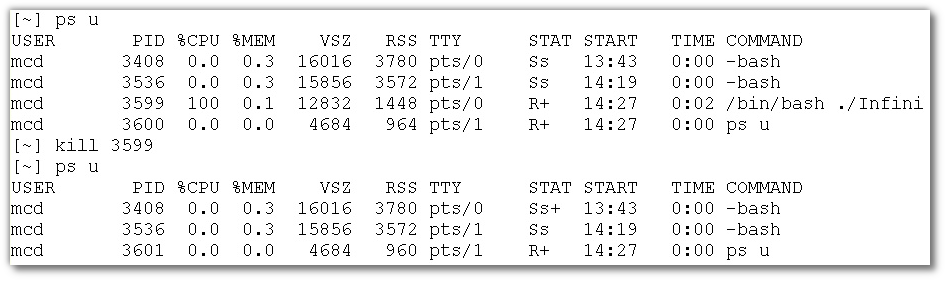
\includegraphics[width=1\linewidth,height=0.8\textheight,keepaspectratio=true]{/home/cuvelier/Documents/ESI/Java/2016-2017/DEV1Q2/notes/DEV1Q2/TDLinux/fr/image/capt1.png}
						\end{center}
                
                    \caption[ps et kill]{ps et kill}
                \end{figure}
                    
					\begin{itemize}
				
			\item \verb@kill 3599@
						envoie au processus de PID 
						\verb@3599@
						le signal n\textdegree  15 (SIGTERM, signal par d\'efaut),
						qui demande au processus de se terminer.
					
			\item \verb@kill -SIGKILL 3599@ 
						ou \verb@kill -9 3599@
						envoie explicitement le signal n\textdegree  9 (SIGKILL) au processus 
						\verb@3599@; ceci le tuera.
					
			\item 
						La touche clavier \verb@Ctrl-c@
						envoie le signal n\textdegree  2 (SIGINT) au processus li\'e au terminal
						et a comme effet de le
						\textbf{terminer}.
					
			\item 
						La touche clavier \verb@Ctrl-z@
						envoie le signal n\textdegree  20 (SIGTSTP) au processus li\'e au terminal
						et a comme effet de le 
						\textbf{suspendre}.
						Ce dernier reste donc dans le syst\`eme.
					
			\item 
						Pour obtenir la liste de tous les signaux :
						\verb@kill -l@ ou 
						encore \verb@man 7 signal@.
					
					\end{itemize}
				
            \par
        
			
		\subparagraph{Exp\'erimentation - La boucle infinie} 
		
					\textcolor{white}{.} \par
				
            \par
        
					\begin{enumerate}
				
			\item 
						\'Ecrivez un programme minimal 
						contenant une boucle infinie
						\begin{Java}
	while(true){}
						\end{Java}
			\item 
						Visualisez vos processus en cours en utilisant la commande 
						\verb@ps u@.
					
			\item 
						Ouvrez une seconde fen\^etre putty, et ex\'ecutez-y 
						votre boucle infinie.
						Ex\'ecutez \`a nouveau la commande 
						\verb@ps u@
						dans la premi\`ere fen\^etre.
					
			\item 
						Retrouvez le processus correspondant au programme 
						qui cycle (son PID)
						et tuez-le en utilisant la commande kill
						avec les bons param\`etres. Quel nom a le programme \`a tuer ?
						
            \par
        
						Sur linux1,
						le syst\`eme tue les processus apr\`es un temps d\'efini
						d'utilisation du CPU (timeout). Il se pourrait donc
						qu'il s'arr\^ete avant l'effet de votre action ;
						ce n'est pas le moment de s'endormir ;-).
						
            \par
        
			\item 
						Lancez une deuxi\`eme ex\'ecution et suspendez votre programme 
						par \verb@Ctrl-z@.
						V\'erifiez l'\'etat du processus stopp\'e par la commande 
						\verb@ps@
						(\verb@man ps@ et recherchez 
						la signification du champ 
						\verb@STAT@).
					
			\item 
						Reprenez le processus interrompu en envoyant le signal 
						SIGCONT (via la commande kill) 
						et v\'erifiez son nouvel \'etat avant qu'il ne soit \'eject\'e par 
						le syst\`eme \`a cause du \guillemotleft timeout\guillemotright .
					
			\item 
						Une deuxi\`eme mani\`ere de reprendre un processus suspendu
						est de taper la commande
						\verb@fg num@ 
						(faites un \verb@man bash@),
						cela doit \^etre fait dans la console dans laquelle vous 
						avez tap\'e \verb@Ctrl-z@.
						Le num\'ero \verb@num@
						est fourni par le syst\`eme lorsque le processus 
						a \'et\'e suspendu par \verb@Ctrl-z@.
						
            \par
        
						Essayez aussi \verb@fg@ 
						pour reprendre le dernier processus suspendu.
						
            \par
        
					\end{enumerate}
				\section{Conclusion}\subsection{F\'elicitations}
					Vous \^etes arriv\'es au bout de ce premier TD.
        				
            \par
        
					Avant de quitter le laboratoire, n'oubliez pas de 
					quitter proprement la connexion avec \verb@linux1@
						(\,\verb|exit|\,).
					et d'\'eteindre l'ordinateur ou de vous d\'eloguer.
					
            \par
        
					Attention, afin d'arriver au laboratoire dans les meilleures conditions, il est 
					bien de revoir la mati\`ere qui sera mise en pratique.
					C'est pourquoi nous vous fournissons quelques \textbf{exercices pr\'eparatoires} \`a faire \`a la maison 
					pour vous permettre d'\'evaluer si vous \^etes pr\^et.
					Afin de v\'erifier que vous pr\'eparez bien ces exercices, une
					\textbf{interrogation}
					sera faite avant de d\'emarrer chaque labo.
				
            \par
        
					\`A la semaine prochaine et soyez \`a l'heure !
				
            \par
        
				\end{document}
			